\section{Radio Interferometry and the Inverse Problem in Astronomy}\label{intro}
Radio instruments in Astronomy require a sub-arcsecond angular resolution. For a single dish antenna, the angular resolution is $ \theta \approx \lambda / D$ radians, which leads to impossibly large diameters for radio wavelengths. This has lead to the use of Interferometers where several smaller antennas act as a single large instrument. 

However, calculated the observed image for interferometers is not trivial. It measures a limited set of Fourier components (Visibilities) of the observed image. image reconstruction from undersampled fourier components(called 'Visibilities' in Radio Astronomy). The Inverse Problem. Radio Astronomy has come up with the CLEAN class Algorithms\cite{hogbom1974aperture} \cite{schwab1984relaxing} \cite{rich2008multi}\cite{rau2011multi} that work well in practice for current radio interferometers.

Theory of Compressed Sensing can retrieve Signals Below Nyquist-Shannon Rates that has theoretical guarantees, can model the effects of new large-scale interferometers (SKA). Active Field of Research





At first glance, the image reconstruction does not seem hard. Since the interferometer measures Fourier components, one can calculate the inverse Fourier transform. The Fourier Measures are incomplete, therefore only a "dirty" image can easily be retrieved. The CLEAN \cite{hogbom1974aperture} algorithm was created to clean up the dirty image and. Over the years the original CLEAN algorithm has been extended and modified, but the general idea stayed the same (Cotton-Schwab-CLEAN \cite{schwab1984relaxing}, MS-CLEAN \cite{rich2008multi}, MS-MFS-CLEAN\cite{rau2011multi})

The theory of Compressed Sensing \cite{candes2006robust} \cite{donoho2006compressed} is another way of looking at the problem. It says we can fully reconstruct the true image if the signal is compressible.

Compressed Sensing, a formula with theoretical guarantees that can handle plausible images.

The remainder of this chapter will introduce basics in Interferometry, the state of the art image reconstruction and an introduction to compressed sensing. Active research field in radioastronomy. It tries to get an algorithm ready for SKA and different approaches get put forward(Purify, SASIR)

\subsection{Simplified Inverse Problem}
The Measurements in Radio Astronomy are complex, but for current Instruments the Inverse problem can be simplified with assumptions. In the section \ref{radio} goes into details what the assumptions are and how they won't hold true for future instruments.

\begin{figure}[h!]
	\centering
	\begin{subfigure}[b]{0.3\linewidth}
		 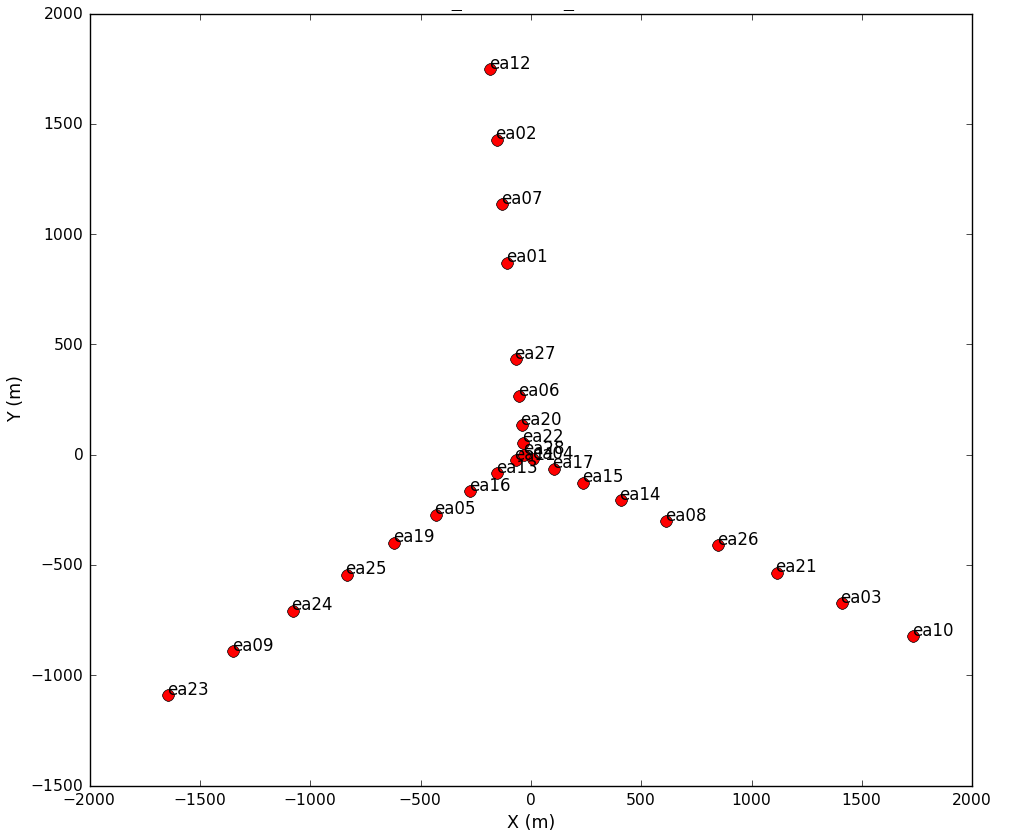
\includegraphics[width=\linewidth]{./chapters/01.intro/img/antennas.png}
		 \caption{Antenna Configuration}
	\end{subfigure}
	\begin{subfigure}[b]{0.3\linewidth}
		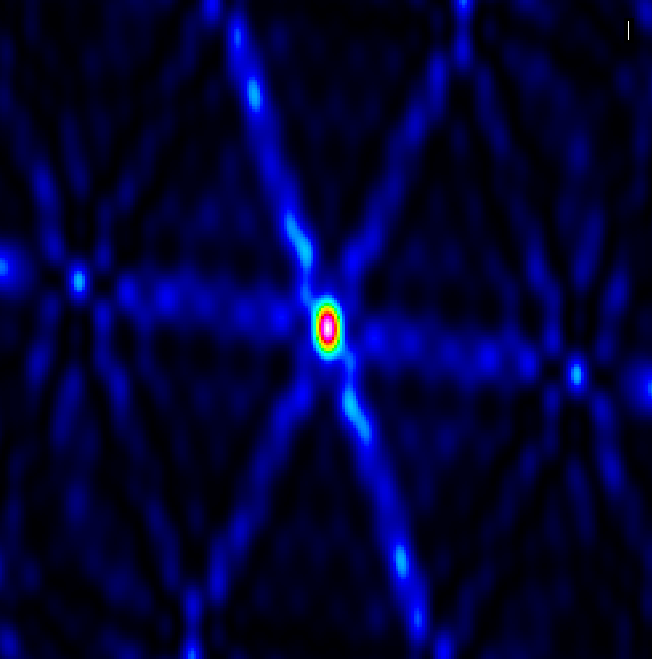
\includegraphics[width=\linewidth]{./chapters/01.intro/img/PSF.png}
		\caption{UV Coverage}
	\end{subfigure}
	\begin{subfigure}[b]{0.3\linewidth}
	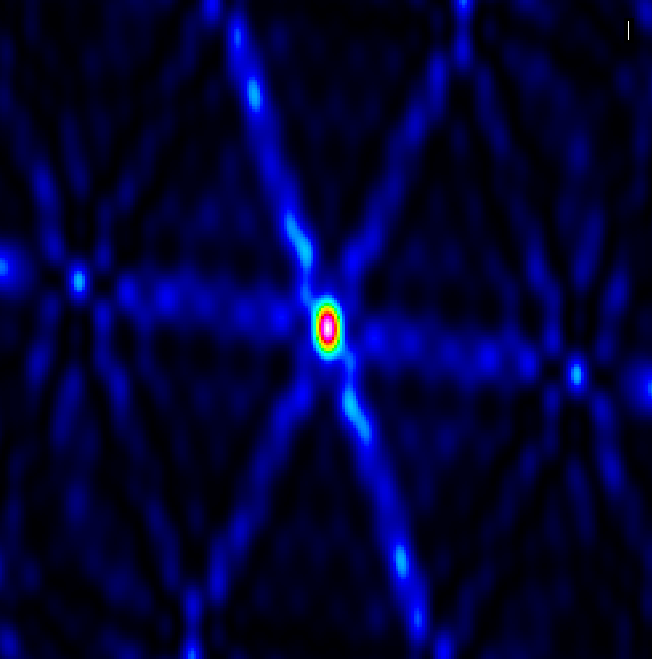
\includegraphics[width=\linewidth]{./chapters/01.intro/img/PSF.png}
	\caption{Point Spread Function}
	\end{subfigure}
	\caption{The Antenna Configuration sets up the UV Coverage. The UV Coverage dictates the Point Spread Function.}
	\label{intro:ANT_UV_PSF}
\end{figure}

\ref{intro:ANT_UV_PSF}
Antennas, Combinatorial Baselines,. The Further away two antennas are, [the higher the frequency?]. Antenna Configuration Leads to the UV Plane. Measures Amplitude and Phase. The Inverse Fourier Transform would produce the image, if the UV Plane was completely sampled. Since it is undersampled, the image resulting from the inverse Fourier Transform contains artefacts. Luckily, the artefacts can be estimated: We know the UV Plane How the artefacts transform the image is represented in the Point Spread Function (PSF). The PSF represents instrumental effects.

\begin{figure}[h!]
	\centering
	\begin{subfigure}[b]{0.3\linewidth}
		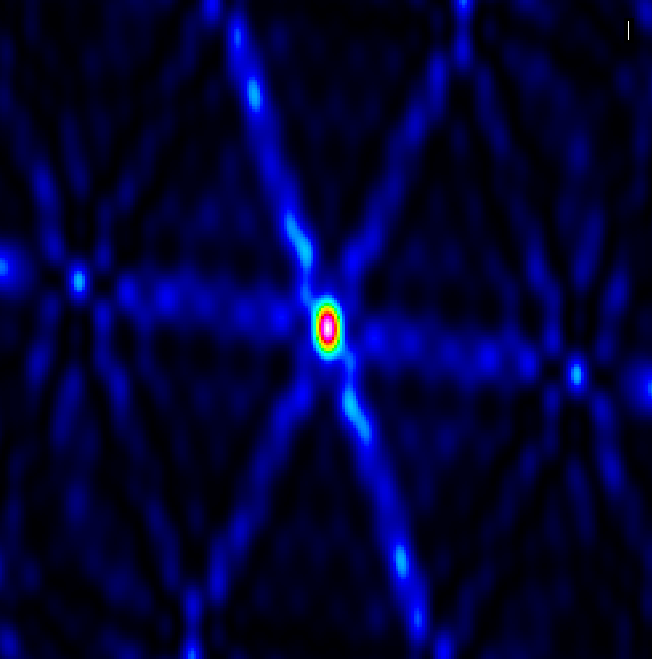
\includegraphics[width=\linewidth]{./chapters/01.intro/img/PSF.png}
		\caption{Point Spread Function (PSF).}
	\end{subfigure}
	\begin{subfigure}[b]{0.3\linewidth}
		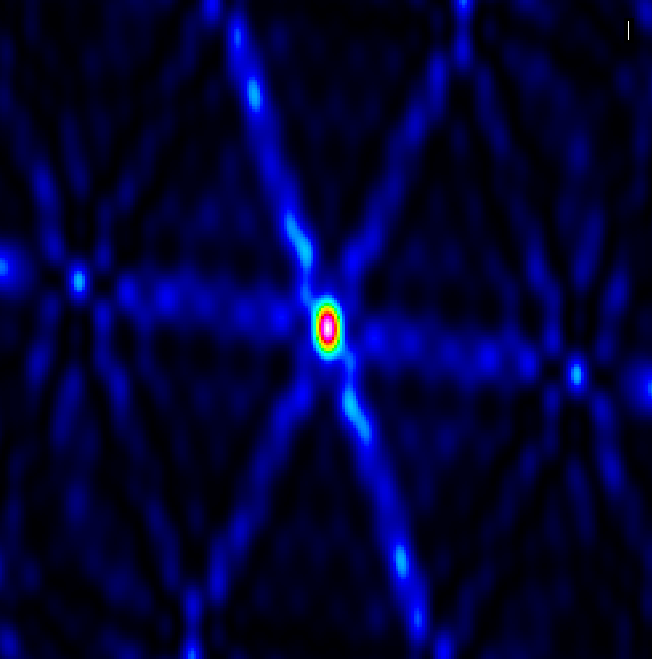
\includegraphics[width=\linewidth]{./chapters/01.intro/img/PSF.png}
		\caption{Dirty image.}
	\end{subfigure}
	\begin{subfigure}[b]{0.3\linewidth}
		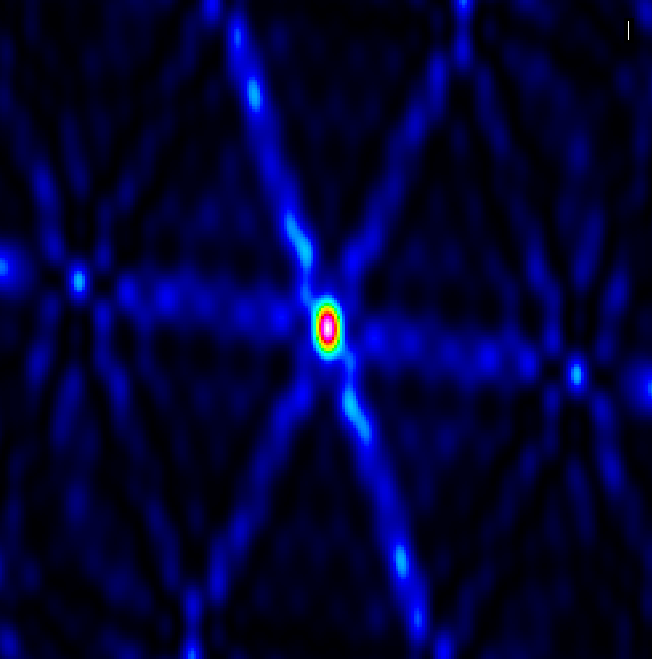
\includegraphics[width=\linewidth]{./chapters/01.intro/img/PSF.png}
		\caption{True image of the sky.}
	\end{subfigure}
	\caption{The Inverse Problem: Finding the true image of the sky when only the PSF and the observed image are known.}
	\label{intro:inverse_problem}
\end{figure}

Inverse Fourier Transform gets the Observed image(Dirty Image). It has artefacts from the undersampled fourier space. The artefacts are represented in the point spread function. The target is showed in figure \ref{intro:inverse_problem}. With only knowing the Dirty image and the PSF, one tries to retrieve the actual image of the sky.

Convolution with the PSF and the true Image


\subsection{Deconvolution with CLEAN}
Clean follows from the simplified Inverse problem. The dirty image results from the True image getting convolved with the PSF. It searches to deconvolve the dirty image with the PSF and retrieve the actual sky image.

Clean implementation, removing the biggest peak. Early stopping


\begin{equation}\label{intro:deconvolution}
I \star PSF = I_Dirty
\end{equation}
One way of solving the Inverse Problem is to formulate it as a deconvolution as in \eqref{intro:deconvolution}. The image $I$ is what the Interferometer would observe if the UV-Space was fully sampled. But since the UV-Space is undersampled, $I$ gets convolved with the Point Spread Function $PSF$ and the Interferometer observes the Fourier of components of the dirty Image $I_D$. After the Inverse Fourier Transform, the CLEAN algorithms deconvolve $I_D$ with the $PSF$ to find the actual Image.


\subsection{Compressed Sensing Formulation}

clean in CS formulation. Prior knowledge of the sky. Theory of compressed sensing states that we can retrieve the true image potentially below the Nyquist Shannon Rate.

Freedom to find a good representation, Prior can be learned. SKA's inverse problem will be larger and more challenging, because the assumptions that lead to the simplified inverse problem and by extend to CLEAN do not hold true.

Problem with speed, scale of SKA 

Optimization algorithms. A formulation which get distributed.


\begin{equation}\label{intro:underdetermined}
\begin{split}
Fx = y
\end{split}
\begin{split}
x &\in \mathcal{R}^n\\
y &\in \mathcal{C}^m\\
2m &< n
\end{split}
\end{equation}
Another way of looking at the inverse problem is to formulate it as the solution to an underdetermined system. \eqref{intro:underdetermined}. In our case, $y$ are the observed Fourier components, $x$ is the reconstructed image and $F$ is the Fourier Transform. We try to find $x$ that explain the observations $y$, but since it is an under determined system, there are multiple solutions. The intuitive way to solve it is to increase the number of observations until we have a fully-determined system. However, this is not necessary. With the theory of Compressive Sensing one can find the correct solution by exploiting the fact that $x$ is compressible.

It turns out that many natural signals are compressible. A picture taken by an ordinary camera produces megabytes of data, but after compression only a fraction of the original need to stored. JPEG2000 uses the Wavelet Transform and only needs to store a limited number of Wavelet coefficients. More formally, if $W$ is the Wavelet transform and $e$ a natural Image, $We = \alpha$. $\alpha$ are the wavelet coefficients. Since natural images are compressible in the wavelet domain, $\alpha$ is sparse (contains mostly zeroes) and can be stored using less space than the image $e$.

Coming back to the original underdetermined system \eqref{intro:underdetermined}, we introduce a Dictionary $D$ which contains our basis functions. We assume that $x$ is compressible using the Dictionary: $D\alpha = x$ and $\alpha$ has only a few non-zero entries. Instead of solving \eqref{intro:underdetermined} directly, we substitute $x$ with $D\alpha$ and search for the solution that has the fewest non-zero elements in $\alpha$. We arrive at the minimization problem \eqref{intro:ssparseland}, where $\mathit{ind}()$ is the indicator function. 

S- Compressible. Under what circumstance is $D\tilde{\alpha} = x$. In compressed Sensing states that if we have a "good" dictionary, i.e. one where $x$. Also there are few limitations on $D$. It can be the Wavelet transform, Fourier Transform, or even a combination of the two.

\begin{equation}\label{intro:ssparseland}
\tilde{\alpha} =  \underset{\alpha}{arg min} \: \mathit{ind}(D\alpha) \quad s. t. \quad FD\alpha = y
\end{equation}

Non-convex optimization, real environment has noise. It can be shown that the L1 norm approximates the indicator function.


\begin{equation}\label{intro:sparseland}
\begin{split}
x  =  D_{\alpha}
\end{split}
\quad , \quad
\begin{split}
x &\in \mathcal{R}^n\\
\alpha &\in \mathcal{R}^k\\
D &\in \mathcal{R}^{n \times k}
\end{split}
\quad with \quad
\begin{split}
n \ll k
\end{split}
\end{equation}

Plausible Image, sparsity

\begin{equation}\label{cs:noiseless}
\tilde{\alpha} =  \underset{\alpha}{arg\: min}
\end{equation}

